%% LyX 2.4.3 created this file.  For more info, see https://www.lyx.org/.
%% Do not edit unless you really know what you are doing.
\documentclass[11pt,oneside,czech,american]{book}
\usepackage[T1]{fontenc}
\usepackage[utf8]{inputenc}
\setcounter{secnumdepth}{3}
\usepackage{url}
\usepackage{amsmath}
\usepackage{amsthm}
\usepackage{amssymb}
\usepackage{graphicx}
\usepackage{minted}
\usepackage[a4paper]{geometry}
\geometry{verbose,tmargin=4cm,bmargin=3cm,lmargin=3cm,rmargin=2.5cm,headheight=0.8cm,headsep=1cm,footskip=0.5cm}
\pagestyle{headings}
\usepackage{setspace}

\makeatletter
%%%%%%%%%%%%%%%%%%%%%%%%%%%%%% Textclass specific LaTeX commands.
\newenvironment{lyxlist}[1]
	{\begin{list}{}
		{\settowidth{\labelwidth}{#1}
		 \setlength{\leftmargin}{\labelwidth}
		 \addtolength{\leftmargin}{\labelsep}
		 \renewcommand{\makelabel}[1]{##1\hfil}}}
	{\end{list}}

%%%%%%%%%%%%%%%%%%%%%%%%%%%%%% User specified LaTeX commands.
%% Font setup: please leave the LyX font settings all set to 'default'
%% if you want to use any of these packages:

%% Use Times New Roman font for text and Belleek font for math
%% Please make sure that the 'esint' package is turned off in the
%% 'Math options' page.
\usepackage[varg]{txfonts}

%% Use Utopia text with Fourier-GUTenberg math
%\usepackage{fourier}

%% Bitstream Charter text with Math Design math
%\usepackage[charter]{mathdesign}

%%---------------------------------------------------------------------

%% Make the multiline figure/table captions indent so that the second
%% line "hangs" right below the first one.
%\usepackage[format=hang]{caption}

%% Indent even the first paragraph in each section
\usepackage{indentfirst}

%%---------------------------------------------------------------------

\usepackage{pdfpages}

%%---------------------------------------------------------------------

%% Disable page numbers in the TOC. LOF, LOT (TOC automatically
%% adds \thispagestyle{chapter} if not overriden
%\addtocontents{toc}{\protect\thispagestyle{empty}}
%\addtocontents{lof}{\protect\thispagestyle{empty}}
%\addtocontents{lot}{\protect\thispagestyle{empty}}

%% Shifts the top line of the TOC (not the title) 1cm upwards
%% so that the whole TOC fits on 1 page. Additional page size
%% adjustment is performed at the point where the TOC
%% is inserted.
%\addtocontents{toc}{\protect\vspace{-1cm}}

%%---------------------------------------------------------------------

% completely avoid orphans (first lines of a new paragraph on the bottom of a page)
\clubpenalty=9500

% completely avoid widows (last lines of paragraph on a new page)
\widowpenalty=9500

% disable hyphenation of acronyms
\hyphenation{CDFA HARDI HiPPIES IKEM InterTrack MEGIDDO MIMD MPFA DICOM ASCLEPIOS MedInria}

%%---------------------------------------------------------------------

%% Print out all vectors in bold type instead of printing an arrow above them
\renewcommand{\vec}[1]{\boldsymbol{#1}}

% Replace standard \cite by the parenthetical variant \citep
%\renewcommand{\cite}{\citep}

\makeatother
\bibliography{export}
\bibliographystyle{unsrt}
\usepackage{biblatex}
\usepackage{babel}
\usepackage{hyperref}
\begin{document}
\def\documentdate{August 4, 2025}

%%\def\documentdate{\today}

\pagestyle{empty}
{\centering

\noindent{}%
\begin{minipage}[c]{3cm}%
\begin{center}

\includegraphics[width=3cm,keepaspectratio,height=3cm]{Images/TITLE/cvut}
\par\end{center}%
\end{minipage}%
\begin{minipage}[c]{0.6\linewidth}%
\begin{center}
{\large\textsc{Czech Technical University in Prague}}{\large}\\
{\large Faculty of Nuclear Sciences and Physical Engineering}
\par\end{center}%
\end{minipage}%
\begin{minipage}[c]{3cm}%
\begin{center}

\includegraphics[width=3cm,keepaspectratio,height=3cm]{Images/TITLE/fjfi}
\par\end{center}%
\end{minipage}

\vspace{3cm}

{\huge\textbf{Web application for team work organization}}{\huge\par}

\vspace{1cm}

\selectlanguage{czech}%
{\huge\textbf{Webová aplikace pro organizaci týmové práce}}{\huge\par}

\selectlanguage{american}%
\vspace{2cm}

{\large Bachelor's Degree Project}{\large\par}

}

\vfill{}

\begin{lyxlist}{MMMMMMMMM}
\begin{singlespace}
\item [{Author:}] \textbf{Kirill Borodinskiy}
\item [{Supervisor:}] \textbf{doc. Ing. Miroslav Virius, CSc.}
\item [{Academic~year:}] 2024/2025
\end{singlespace}
\end{lyxlist}

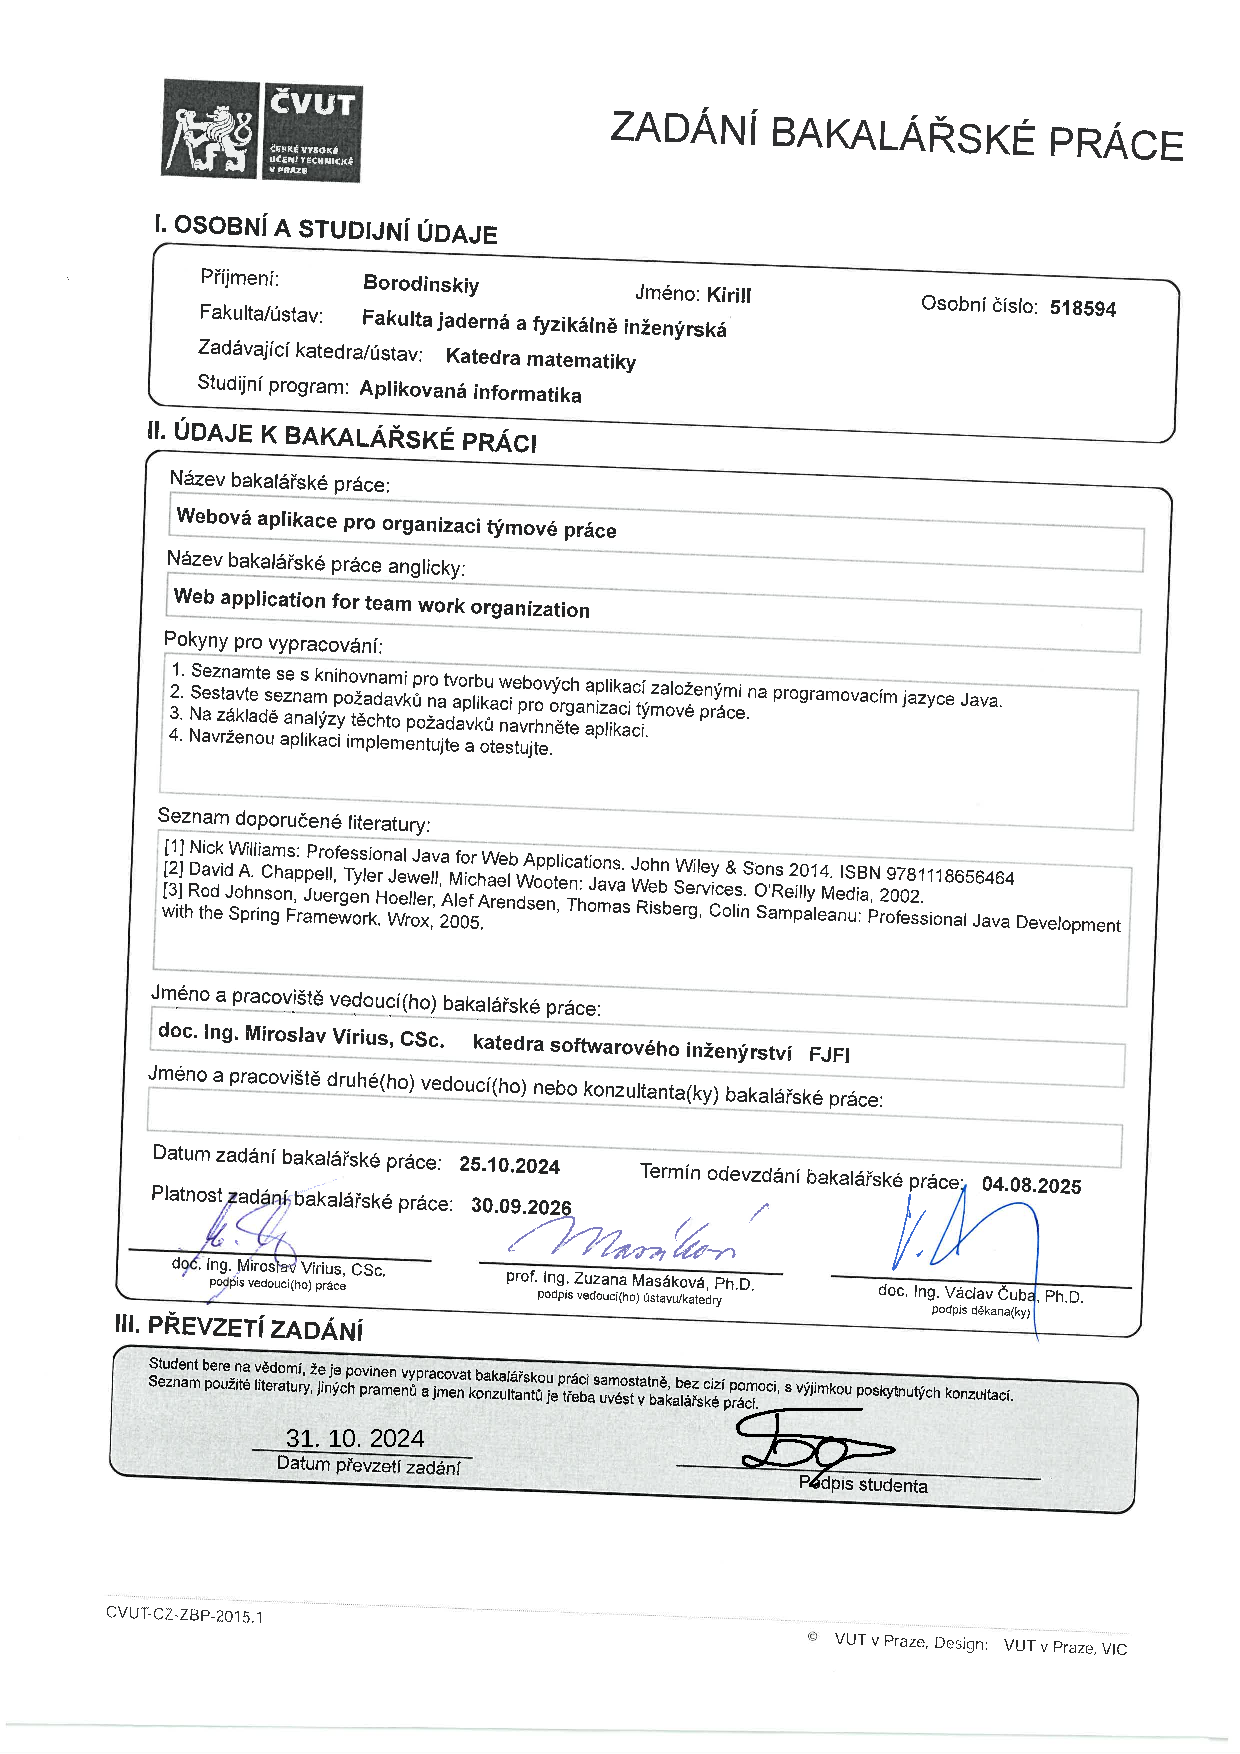
\includepdf[]{BPZADANI.pdf}

\noindent{\Large\emph{Acknowledgment:}}{\Large\par}

\noindent I would like to thank my mother Elena and my girlfriend Anastasiia for their moral support.
I would like to thank my supervisor, Miroslav Virius, for their help in organization of my bachelor's thesis project.

\vfill

\noindent{\Large\emph{Author's declaration:}}{\Large\par}

\noindent I declare that this Bachelor's Degree Project is entirely
my own work and I have listed all the used sources in the bibliography.
AI tools were used in full accordance with the guidelines established
by CTU in Prague.

\bigskip{}

\noindent Prague, \documentdate\hfill{}Kirill Borodinskiy

\vspace{2cm}

\newpage{}

\selectlanguage{czech}%
\begin{onehalfspace}
\noindent\emph{Název práce:}

\noindent\textbf{Webová aplikace pro organizaci týmové práce}
\end{onehalfspace}

\bigskip{}

\noindent\emph{Autor:} Kirill Borodinskiy

\bigskip{}

\noindent\emph{Studijní program:} Celý název studijního programu
(nikoliv zkratka)\bigskip{}

\noindent\emph{Specializace:} Celý název specializace (Pokud se studijní
program nedělí na specializace, tuto řádku odstranit.)

\bigskip{}

\noindent\emph{Druh práce:} Bakalářská práce

\bigskip{}

\noindent\emph{Vedoucí práce:}doc.
Ing.
Miroslav Virius, CSc., DrSc.,
pracoviště školitele (název instituce, fakulty, katedry)

\bigskip{}

\bigskip{}

\noindent\emph{Abstrakt:} Abstrakt max.
na 10 řádků.
Abstrakt max.
na 10 řádků.
Abstrakt max.
na 10 řádků.
Abstrakt max.
na 10 řádků.
Abstrakt max.
na 10 řádků.
Abstrakt max.
na 10 řádků.
Abstrakt max.
na 10 řádků.
Abstrakt max.
na 10 řádků.
Abstrakt max.
na 10 řádků.
Abstrakt max.
na 10 řádků.
Abstrakt max.
na 10 řádků.
Abstrakt max.
na 10 řádků.
Abstrakt max.
na 10 řádků.
Abstrakt max.
na 10 řádků.
Abstrakt max.
na 10 řádků.
Abstrakt max.
na 10 řádků.
Abstrakt max.
na 10 řádků.
Abstrakt max.
na 10 řádků.
Abstrakt max.
na 10 řádků.
Abstrakt max.
na 10 řádků.
Abstrakt max.
na 10 řádků.
Abstrakt max.
na 10 řádků.
Abstrakt max.
na 10 řádků.
Abstrakt max.
na 10 řádků.
Abstrakt max.
na 10 řádků.
Abstrakt max.
na 10 řádků.
Abstrakt max.
na 10 řádků.
Abstrakt max.
na 10 řádků.
Abstrakt max.
na 10 řádků.

\bigskip{}

\noindent\emph{Klíčová slova:} klíčová slova (nebo výrazy) seřazená
podle abecedy a oddělená čárkou

\selectlanguage{american}%
\vfill{}
~

\begin{onehalfspace}
\noindent\emph{Title:}

\noindent\textbf{Title of the Work}
\end{onehalfspace}

\bigskip{}

\noindent\emph{Author:} Kirill Borodinskiy

\bigskip{}

\noindent\emph{Abstract:} Max.
10 lines of English abstract text.
Max.
10 lines of English abstract text.
Max.
10 lines of English abstract
text.
Max.
10 lines of English abstract text.
Max.
10 lines of English
abstract text.
Max.
10 lines of English abstract text.
Max.
10 lines
of English abstract text.
Max.
10 lines of English abstract text.
Max.
10 lines of English abstract text.
Max.
10 lines of English abstract
text.
Max.
10 lines of English abstract text.
Max.
10 lines of English
abstract text.
Max.
10 lines of English abstract text.
Max.
10 lines
of English abstract text.
Max.
10 lines of English abstract text.
Max.
10 lines of English abstract text.
Max.
10 lines of English abstract
text.
Max.
10 lines of English abstract text.
Max.
10 lines of English
abstract text.
Max.
10 lines of English abstract text.
Max.
10 lines
of English abstract text.
Max.
10 lines of English abstract text.
Max.
10 lines of English abstract text.
Max.
10 lines of English abstract
text.
Max.
10 lines of English abstract text.

\bigskip{}

\noindent\emph{Key words:} keywords in alphabetical order separated
by commas

\newpage{}

\pagestyle{plain}

\tableofcontents{}

\newpage{}







\chapter{Introduction}\label{ch:introduction}
\section*{Motivation}
Efficient team schedule planning is a complex challenge, particularly in organizations that require real-time coordination and resource management.
Existing scheduling services often have significant limitations, such as proprietary nature, lack of customization, and dependence on third-party infrastructure.
This project aims to develop a self-hosted open-source booking system designed for organizations that need a private, adaptable scheduling solution.
The system will provide a web-based interface where users can:
\begin{itemize}
    \item Make and manage reservations
    \item Check real-time room availability
    \item  Filter bookings by person or room
    \item View all reservations on a centralized calendar
\end{itemize}

The backend will be built using the Spring Framework, ensuring scalability, security, and ease of integration with existing infrastructure.
Unlike cloud-based alternatives, this system will store all data locally, giving organizations complete privacy and control over scheduling information.
By combining flexibility, transparency, and data privacy, this project can provide a practical alternative to commercial scheduling tools, empowering organizations with greater autonomy and customization options.
\addcontentsline{toc}{section}{Motivation}


\pagestyle{headings}
Here we will talk about why the calendar is needed

Firstly, lets take a look at the current solution used by my university,CTU. Rozvrh.fjfi.cvut.cz is a website where students can see their schedule.
\section{The current solution}\label{sec:the-current-solution}
\begin{figure}[h]
  \centering
  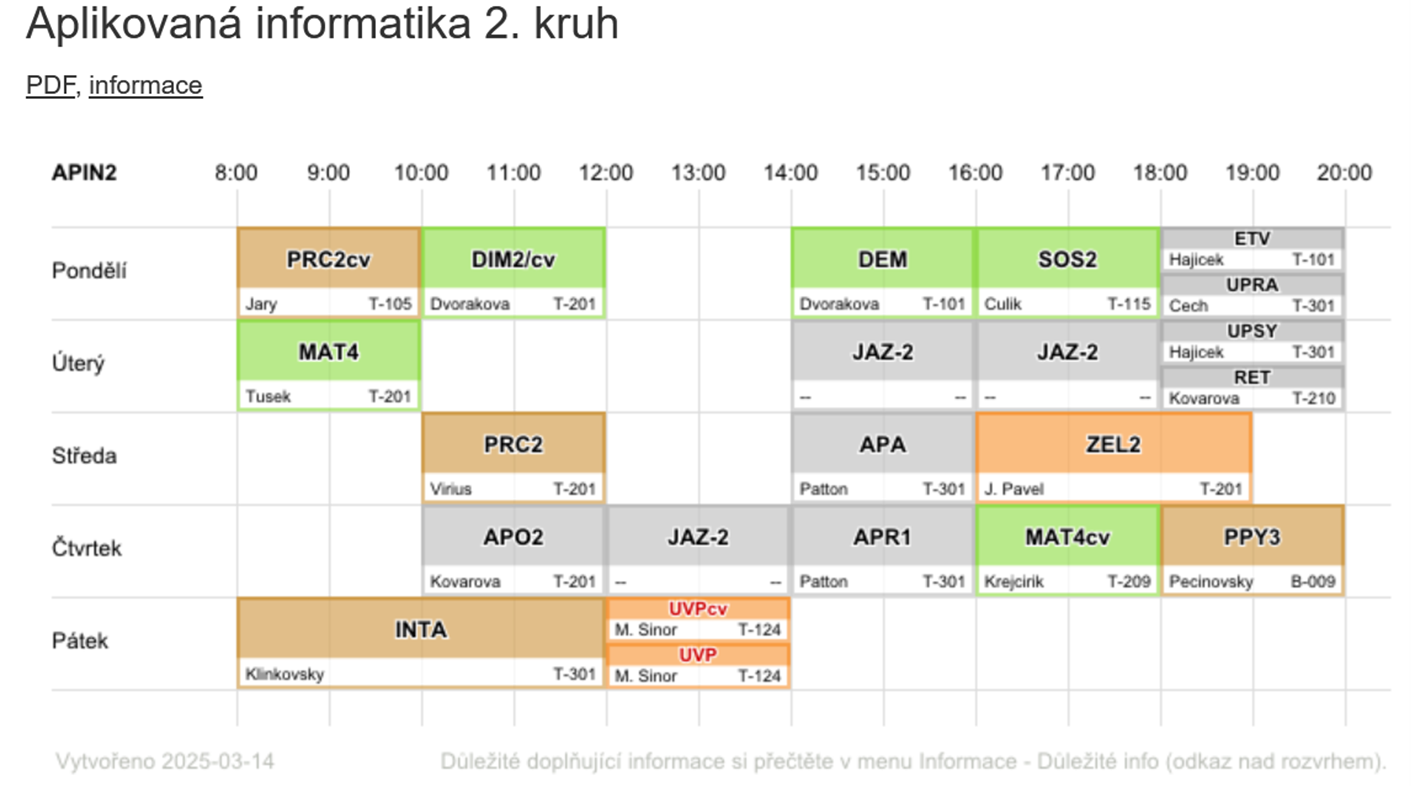
\includegraphics[width=0.6\textwidth]{img}
  \caption{Screenshot of the current solution}
  \label{fig:rozvrh}
\end{figure}

It can be seen on~\ref{fig:rozvrh} that while the website completes its main purpose, it is not customizable, which makes it hard to use.
For example, if a student has a class that is from another year or/and program, they have to look at another picture and manually compare them.
From my experience, many students have screenshots on their phones and they cross-out the classes that they are not registered to.
They may have a few screenshots, for different programs or years.
It is not a good solution, as it allows for misunderstandings and mistakes.

This is why a project focused on creating a calendar that is easy to use and customizable is needed.
\section{The solution}\label{sec:the-solution}
\begin{figure}[h]
  \centering
  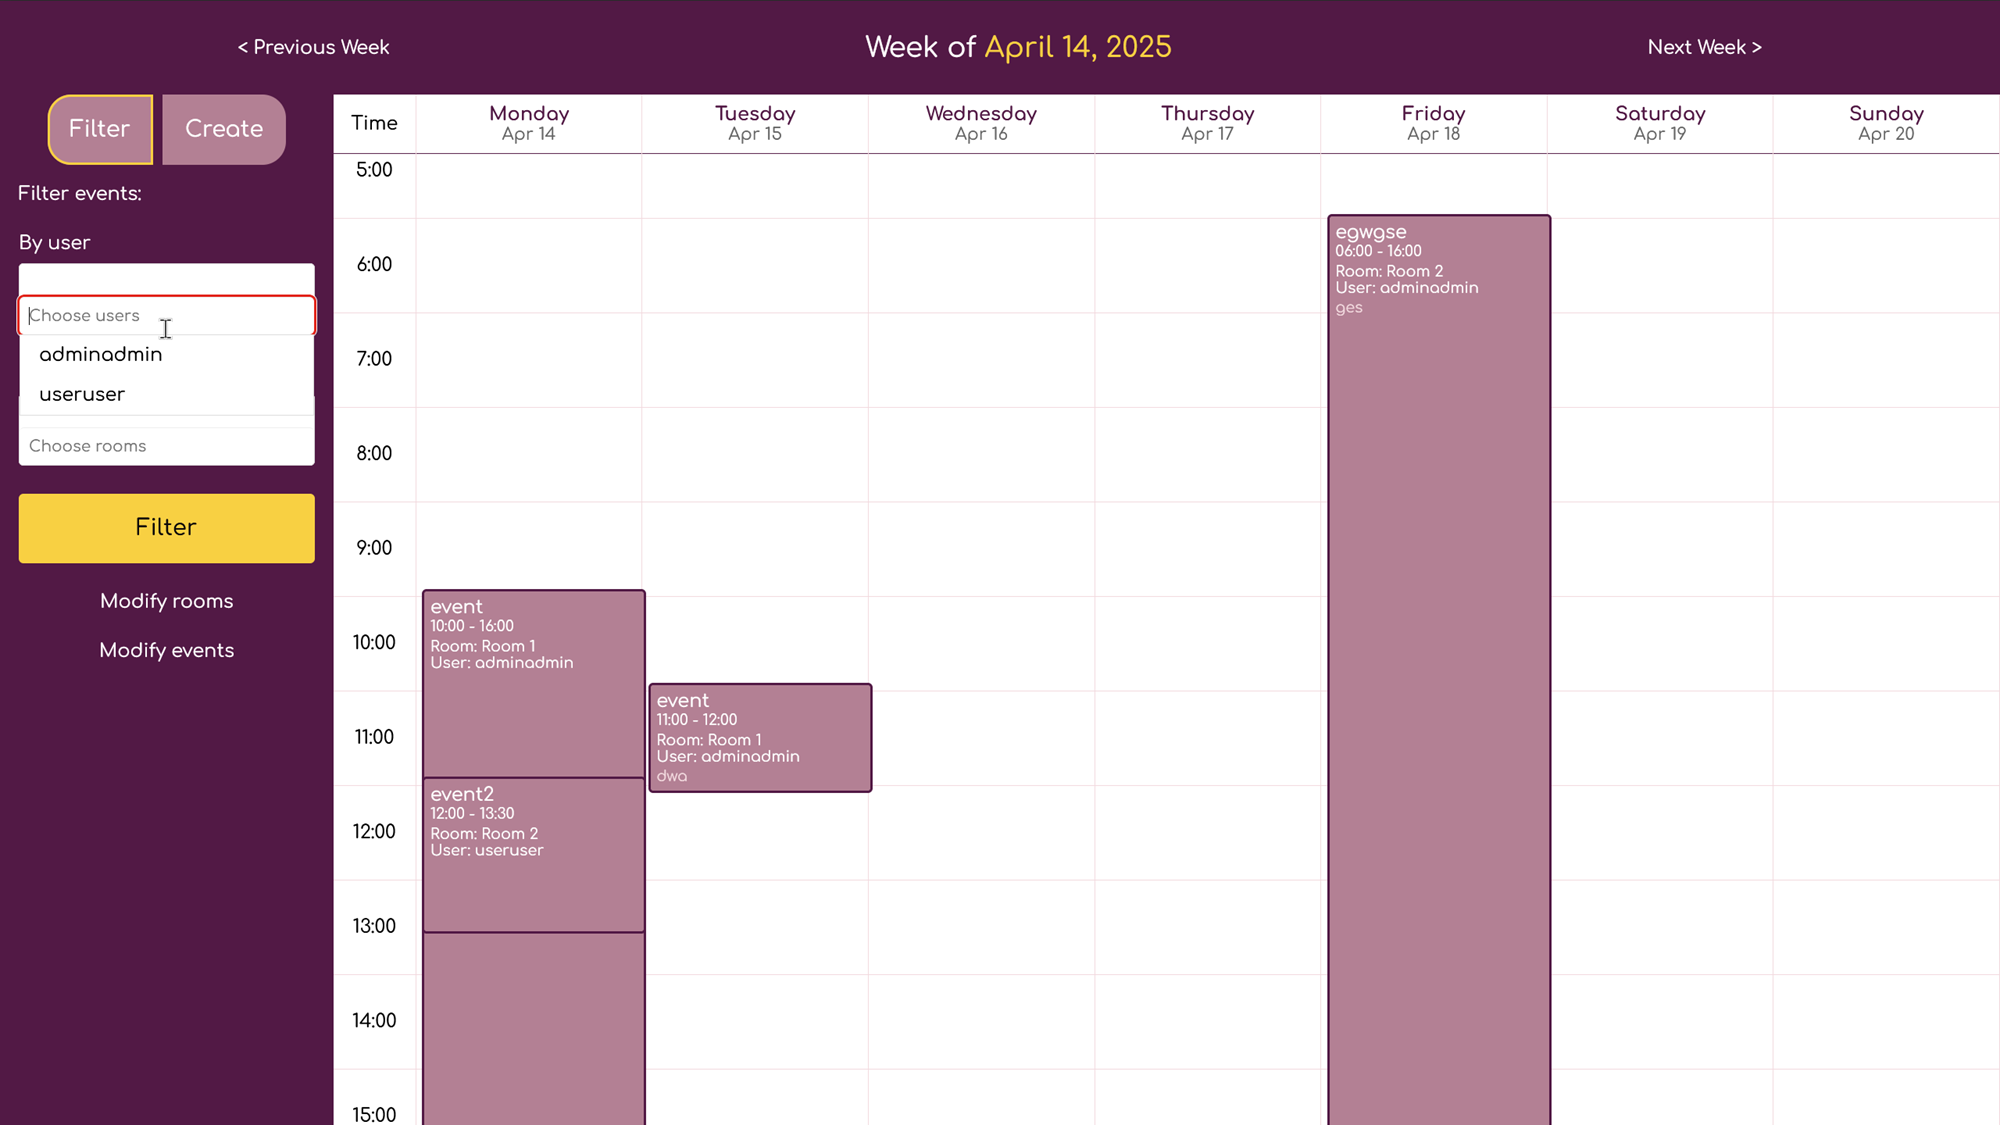
\includegraphics[width=0.6\textwidth]{TeamJob}
  \caption{Screenshot of the new solution}
  \label{fig:TeamJob}
\end{figure}
TeamJob is a web application that allows users to filter exactly what they want to see.
By default, all the events that are happening this week are shown.
The user can filter the events by the room and the person that is assigned to this event.
This allows for a more precise view of the calendar, where the user can see only the events that are important to them.
The user can also move between weeks.
A specific day-view allows the user to see the events that are happening on a specific day, if there are too many events to show them all at once.



\chapter{Methods}\label{ch:methods}
This section will focus on the tools and techniques used to create a web application tShreyashVardhan2024o manage time and space resources of an organization.


\section{Defining the toolbelt}\label{sec:defining-the-toolbelt}
% Расписать все варианты и в итоге выбрать итоговый.
% Расписать всю структуру будущюю.
% Интересные инструменты использованные указать.
% Указать алгортм использованный в приложении.
% Реальные человеческие отзывы сделать.

% Spring Boot vs. Spring vs. C# vs. Django vs. Flask
For the programming language, the options were as follows: Java Spring Boot framework, C\#.NET, and Python's Django and Flask.
C\# was first removed, as learning about it would take a considerable amount of time.
Python's Flask is easy to use, but not customizable enough.
Subsequent analysis, as presented in the study~\cite{ShreyashVardhan2024}, indicates that Spring Boot exhibits superior performance.
Moreover, my familiarity with Java might reduce the time required for development.
Consequently, Spring Boot is selected as the back-end framework.
Spring Boot, which is constructed on the Spring Framework, is recognized as a leading framework within the Java ecosystem due to its widespread popularity.
It streamlines the original Spring Framework, thereby facilitating more straightforward maintenance and expediting deployment procedures.
Henceforth, to maintain clarity, the term Spring Boot shall be used exclusively in reference to both the Spring Framework and Spring Boot.

% Google Web Toolkit vs. Thymeleaf vs. React/other JS
An often-utilized integration of back-end and front-end frameworks with Spring Boot is accomplished through Thymeleaf, a template rendering engine which processes page rendering on the server side, thereby reducing computational demand on the client-side systems.
However, alternative solutions are available, including the currently prevalent React framework along with other JavaScript frameworks.
Opting for these alternatives requires considerable investment in research.
Given my proficiency in HTML, the Thymeleaf template system presents a straightforward learning curve.
Nevertheless, a certain degree of JavaScript is essential for contemporary websites, thereby necessitating its use for handling specific tasks such as requests.


% PostgreSQL vs. NoSQL vs. others
For our database, PostgreSQL was chosen, as it is a popular ACID-compliant database.
ACID stands for:
\begin{itemize}
    \item \textbf{Atomicity}: Transaction is either fully completed, or not, with no in-betweens.
    \item \textbf{Consistency}: Guarantees that a transaction brings the database from a valid state to a valid state.
    \item \textbf{Isolation}: Concurrent transactions do not interfere with each other.
    \item \textbf{Durability}: Once a transaction is committed, it stays committed.
\end{itemize}

\section{Introduction to Spring Boot}\label{sec:introduction-to-spring-boot}

Spring Boot is a tool that allows the programmer to create a web server that uses the Model-View-Controller pattern, MVC for short.

The model is a part responsible for the data logic.
The connection to the database, the processing of the requested data and other back-end transactions are what this part consists of.

The view is a part that displays the data to a user or gathers them from them.
Whether HTML, plain text, or any other format such as our Thymeleaf.

The controller is a connector between the previous two, where the data is additionally processed before being sent into either the database or a client of a user.


\section{Schema of the database}\label{sec:schema-of-the-database}
\begin{figure}[h]
  \centering
  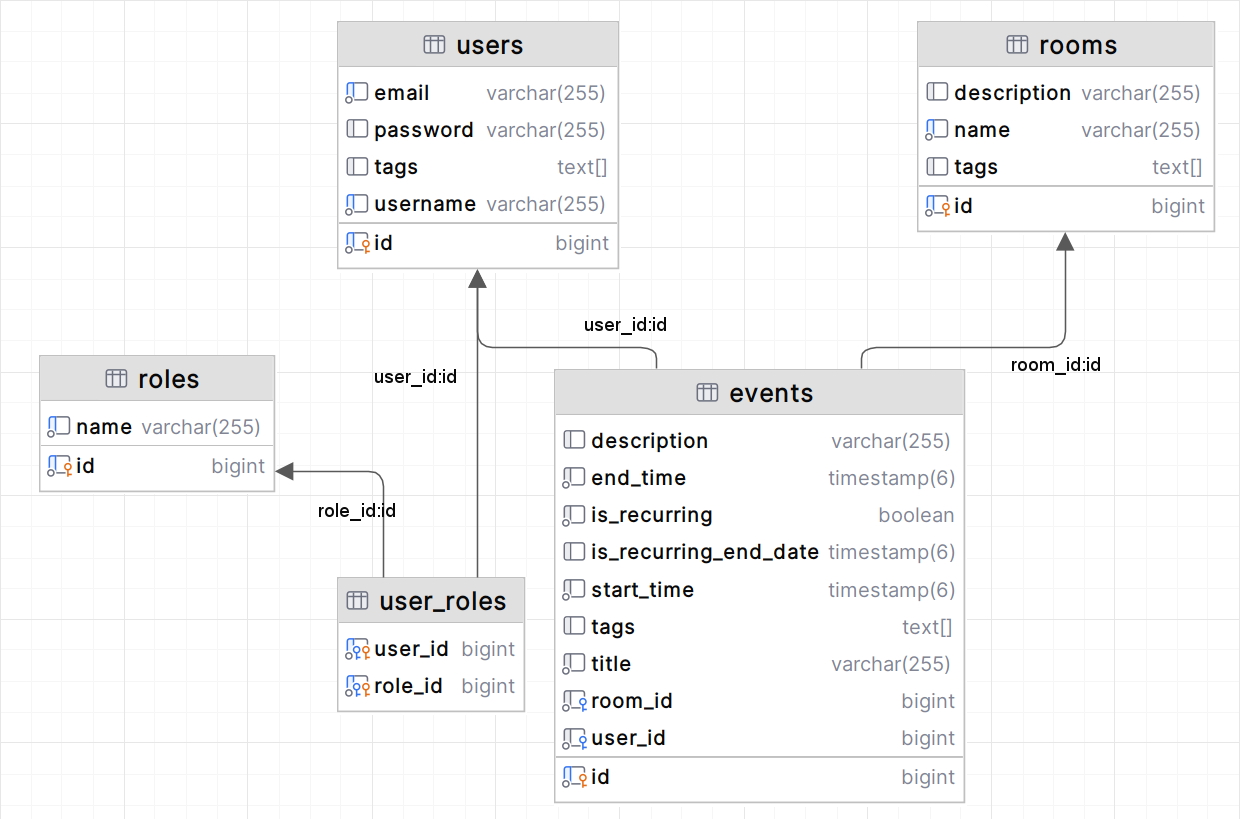
\includegraphics[width=0.6\textwidth]{schemaDB}
  \caption{Schema of the database for the application}
  \label{fig:schemaDB}
\end{figure}

\subsection*{Database \ref{fig:schemaDB} Architecture}

\begin{itemize}
  \item \textbf{users}: Stores user credentials and personal data.
  Each user has a unique \texttt{ID}.

  \item \textbf{roles} \& \textbf{user\_roles}: Implements role-based access control via a many-to-many relation between users and roles.

  \item \textbf{rooms}: Contains information on event locations.
  Each room has a \texttt{name}, \texttt{description} and a unique \texttt{ID}.

  \item \textbf{events}: Represents scheduled activities.
  Includes data such as  \texttt{is\_recurring}, \texttt{title}, \texttt{start\_time} and \texttt{end\_time}.
  Each event references a \texttt{user} and a \texttt{room} that were assigned to this event.

  \item \textbf{users, events }and \textbf{rooms} all contain \texttt{tags} to help categorize them.
\end{itemize}


\newpage%                    NEW PAGE HERE !!!!!!!!!!!!!!!!!!!!!!!!!!!!!!!!!!!!!!!!!!!

\section{The implementation of a Spring Boot application}\label{sec:the-implementation-of-a-spring-boot-application}
In our application, the main controller is CalendarController.
It renders the main page /calendar.
The non-required parameters of a request are: ``\textit{date}'', ``\textit{roomIds}'' and ``\textit{userIds}''.

Parameter \("\)\textit{date}\("\) is simply the day of the week the calendar renders.
If not provided, we use the default value of a current day.

Parameters ``\textit{roomIds}'' and ``\textit{userIds}'' are used to filter out which events the user wants to see in their calendar.
If not provided, events from every room and every user are displayed.

In this controller a week around the current day is generated, all the events that are happening in that week are found and are put into an array that is then sent with the model.


\subsection{Useful tools}\label{subsec:useful-tools}
In this application, \textit{Lombok} was used to reduce the amount of boilerplate code.
It allows for the usage of annotations such as \texttt{@Getter,@Setter} to automatically generate setters and setters for all fields that need them.
In addition, annotations \texttt{@AllArgsConstructor,@NoArgsConstructor} can automatically create the correct construction function for the class.
Finally, \texttt{@Data} combines \texttt{@Getter,@Setter} and some more functions in one annotation, so the classes remain clean and functional.

The use of the tool is demonstrated in the list~\ref{lst:room-class}.
It can be seen that no setter or getter functions are needed, no construction function is needed, and the class looks clean and complete.


\begin{listing}[H]
\begin{minted}{java}
@Data
@Entity
@Table(name = "rooms")
public class Room {
    @Id
    @GeneratedValue(strategy = GenerationType.IDENTITY)
    private Long id;

    @Column(nullable = false, unique = true)
    private String name;

    @Column()
    private String description;

    @Type(io.hypersistence.utils.hibernate.type.array.ListArrayType.class)
    @Column(name = "tags", columnDefinition = "text[]")
    private Set<String> tags = new HashSet<>();
}
\end{minted}
\caption{Lombok-annotated JPA entity}
\label{lst:room-class}
\end{listing}


\newpage%                    NEW PAGE HERE !!!!!!!!!!!!!!!!!!!!!!!!!!!!!!!!!!!!!!!!!!!

\subsection{The architecture of the application}\label{subsec:the-architecture-of-the-application}

The main file responsible for most tasks is CalendarController, where the \texttt{/calendar} endpoint is located.

The \texttt{/calendar} takes 3 non-required parameters.
\begin{itemize}
    \item \textbf{date}: Show the events that happen on the week of the day sent.
    \item \textbf{userIds}: Filter the users shown on the central calendar.
    \item \textbf{roomIds}: Filter rooms displayed in the central calendar.
\end{itemize}
Then, the \texttt{EventRepository} is used to find all the events that are happening in the week of the date sent.
The \texttt{EventRepository} is a Spring Data JPA repository that allows for easy access to the database.
They are split into a list of events that are happening on a specific day, where the days are filtered by comparing the \texttt{userIds} and \texttt{roomIds} with the events that are in the database.
the data inside each event is such:
\begin{itemize}
    \item \textbf{eventId}
    \item \textbf{eventTitle}
    \item \textbf{eventDescription}
    \item \textbf{eventStartTime} - the time when the event starts in LocalDateTime format.
    \item \textbf{eventEndTime}
    \item \textbf{eventRoomId} - the room that is assigned to this event.
    \item \textbf{eventUserId} - the user that is assigned to this event.
    \item \textbf{eventTags} - the tags that are assigned to this event.
    \item \textbf{eventIsRecurring} - if the event is recurring or not.
\end{itemize}
The \texttt{/calendar} then sends such data to \texttt{calendar.html}:
\begin{itemize}
    \item \textbf{userIds} \& \textbf{roomIds} (if supplied from request).
    \item \textbf{selectedDate} (if not provided, current date is used).
    \item \textbf{nextWeek} \& \textbf{previousWeek} to enable navigation within weeks.
    \item \textbf{currentWeekStart}.
    \item \textbf{weekDays} - a list of events that take place on a specific day.
    \item \textbf{eventRepository}, \textbf{userRepository} and \textbf{roomRepository}
\end{itemize}


%Continue describing all endpoints???

\chapter*{Conclusion}

\pagestyle{plain}

\addcontentsline{toc}{chapter}{Conclusion}

Text of the conclusion\ldots{}
\begin{thebibliography}{1}
\bibitem{Allen-Cahn}S. Allen, J. W. Cahn: \emph{A microscopic theory
for antiphase boundary motion and its application to antiphase domain
coarsening}.
Acta Metall., 27:1084-1095, 1979.

\bibitem{CINECA}G. Ballabio et al.: \emph{High Performance Systems
User Guide}.
High Performance Systems Department, CINECA, Bologna,
2005. \url{www.cineca.it}

\bibitem{rumpf3}J. Becker, T. Preusser, M. Rumpf: \emph{PDE methods
in flow simulation post processing}.
Computing and Visualization in
Science, 3(3):159-167, 2000.

\end{thebibliography}

\end{document}
